\documentclass[12pt]{article}
\usepackage[utf8]{inputenc}
\usepackage{amsmath,amssymb}
\usepackage{unicode-math}
\usepackage[T2A]{fontenc}
\usepackage[russian]{babel}
\usepackage{graphicx}
\usepackage{subfigure}
\usepackage{subcaption}
\usepackage{url}
\usepackage{float}


\DeclareGraphicsExtensions{.pdf,.png,.jpg,.svg}
\usepackage{hyperref}
\usepackage{wrapfig}
\usepackage[left=20mm, top=20mm, right=10mm, bottom=20mm]{geometry}

\usepackage{amsmath} 
\usepackage{amsfonts} 
\usepackage{amssymb} 
\usepackage{wasysym} 
\usepackage{fancyhdr}

\pagestyle{fancy}
\fancyhf{}
\lhead{Семинар 9. Ядро. Радиоактивность}
\rhead{\textit{Клименок К.Л., МФТИ 2020}}
\rfoot{\thepage}



\begin{document} 
\title{\textbf{Семинар 9. Ядро. Радиоактивность }}
\author{\textbf{Клименок Кирилл Леонидович}}
\date{10.11.2020}
\maketitle
\section{Теоретическая часть}
Вот мы и закончили ту часть курса, которая отвечает за атомы и теперь мы должны отправиться глубже в атомное ядро.
\begin{figure}[h]
    \centering
    
\includegraphics[width=0.5\textwidth,height=\textheight,keepaspectratio]{Seminar_09/pics/pic_deeper.jpg}
    \caption{Это выражение будет преследовать нас до конца курса квантовой микрофизики}
\end{figure}
\subsection{Свойства ядра}

Начнем мы с того, что попытаемся определить какого же размера у нас ядро и как мы можем это измерить. Тут нам вполне может помочь наша известная модель атома водорода, но вместо электрона можно использовать мюон. Так как он примерно в 200 раз тяжелее, то и его боровский радиус будет в 200 раз меньше (привет задачке из соответствующей недели). А если брать не водород, а что-то потяжелее, например свинец с характерным зарядом около 100 (на деле 82) то получится, что радиус будет еще примерно в 100 раз меньше. Итого получается, что радиус такого атома будет по порядку величины $10^{-10}/2\cdot 10^{4} \text{ м} =5\cdot 10^{-15} \text{ м} = 5 \text{ фм}$. Получили порядок фемтометров. А что тогда с энергией ионизации или энергий переходов? Формула для нее у нас тоже была и она будет выше в $200\cdot 100^2 = 2\cdot 10^6$ раз и это будет масштаб 10 МэВ. Но я напомню, что вся наша теория была построена для точечного ядра, а вот отклонение от <<точечности>> будут давать отклонение в экспериментальных данных и по ним уже можно будет оценить более точный размер. На самом деле, самые внимательные из вас уже заметили некоторое сходство с задачей 4.42 из первого задания. Собственно в ней вы все это и делали. 

В качестве альтернативы этому сложному методу можно попробовать посмотреть на дифракцию электронов на ядре. Тут все немного сложнее, ведь если мы хотим рассмотреть объекты с характерным размером фемтометры, нам надо, чтобы и у электрона длина волны де Бройля была фемтометры. а тогда это уже существенно релятивистский электрон с характерной энергией ГэВ. Кажется, что не очень достижимо, но вот в 1961 году нобелевскую премию вручили Хофштадтеру именно за подобный эксперимент.

Хорошо, с размерами разобрались, теперь о составе. Тут вы, конечно, знаете про протоны и нейтроны. Сильно не буду вдаваться в подробности открытия, просто выдам ссылки на конкретные эксперименты. Для протона это опыты Блеккета, когда в камере Вильсона были обнаружены треки протонов, которые выбивались из ядер азота, а для нейтронов это опыт Чедвика, где также по фотографиям треков были определены его масса и отсутствие заряда.

\subsection{Энергия связи. Формула Вайцзекера и модель жидкой капли}
Начнем с того, что представим как у нас собираются ядра. Пусть у нас есть коробки с отдельными протонами и отдельными нейтронами. Возьмем Z протонов и N нейтронов. Их массы мы знаем с очень хорошей точностью. А теперь совместим их в единое ядро. Оно является стабильным образованием и может существовать какое-то время. На вопрос почему все эти составные части не разлетаются ответ будет <<из-за сильного взаимодействия>>, о нем мы поговорим позже, а пока просто поверим в это. Но если ядро стабильно существует, значит по энергии оно выгоднее чем отдельные его компоненты. Тогда мы можем ввести эту самую энергию связи как различие энергий каждой компоненты ядра и ядра как целого:
\begin{equation}
    E_{\text{св}} = (Z m_pc^2 + N m_nc^2) - M_{\text{ядра}}c^2
\end{equation}
Ну и понятно, что чем больше энергия связи, тем более ядро стабильнее. Но в реальности надо смотреть ни на полную энергию связи, а на удельную (на нуклон). Вот она рисунке \ref{fig:sem_09_link_energy} 
\begin{figure}[h]
    \centering
    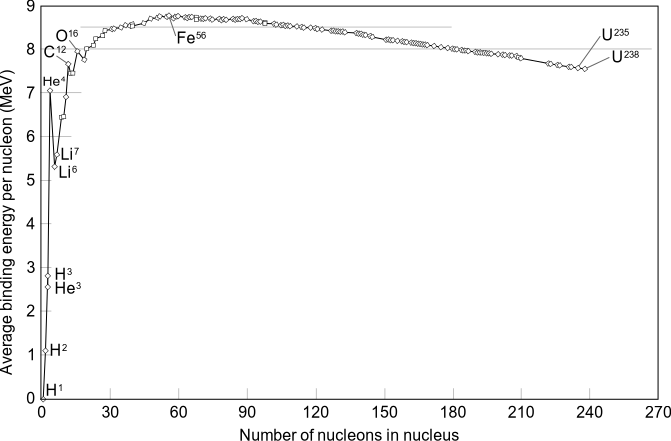
\includegraphics[width=0.7\textwidth,height=\textheight,keepaspectratio]{Seminar_09/pics/pic_binding_energy.png}
    \caption{Энергия связи на нуклон для различных ядер}
    \label{fig:sem_09_link_energy}
\end{figure}
Из характерных особенностей мы видим:
\begin{itemize}
    \item Рост удельной энергии связи для легких ядер с характерными выбросами на ядрах гелия, углерода и кислорода
    \item Характерный максимум на железе в районе 8.5 МэВ
    \item Около линейный спад для более тяжелых ядер
\end{itemize}
Вот тут мы и должны составить какую-то модельку для описания этой картины. И первая модель, которую мы будем рассматривать это жидко-капельная модель. В ней ядро представляется в форме капли <<ядерной жидкости>> и для нее пытаются записать энергию связи. Собственно формула для энергии связи называется формулой Вайцзекера:
\begin{equation}
    E=\alpha A - \beta A^{2/3} - \gamma \dfrac{Z^2}{A^{1/3}} - \epsilon \dfrac{(A/2-Z)^2}{A} + k\dfrac{\delta}{A^{3/4}}
\end{equation}
A -- количество нуклонов, Z -- количество протонов в ядре. Греческие буквы обозначают некоторые подгоночные постоянные. Давайте разберемся с каждым членом отдельно.
\begin{itemize}
    \item $\alpha A$ тут все просто -- чем больше составных частей в ядре тем пропорционально больше энергия связи
    \item $-\beta A^{2/3}$ это влияние поверхности из-за нескомпенсированной силы, действующей на нуклоны на поверхности
    \item $-\gamma \dfrac{Z^2}{A^{1/3}}$ влияние кулоновского отталкивания
    \item $-\epsilon \dfrac{(A/2-Z)^2}{A}$ влияние эквивалентности протонов и нейтронов в сильном взаимодействии
    \item $k\dfrac{\delta}{A^{3/4}}$ $k=1$ для ядер с четным числом протонов и нейтронов, $k=-1$ для ядер с нечетным числом протонов и нейтронов и $k=0$ для остальных случаев
\end{itemize}
Характерные параметры для формулы следующие $\alpha = 14.03, \beta = 13.03, \gamma = 0.53, \epsilon = 77.25, \delta = 34.57$ в МэВ. Эта модель, несмотря на свою простоту, может предсказывать разные интересности, например критерии самопроизвольного распада ядер и состава наиболее стабильных изотопов.

\subsection{Оболочечная модель ядра}
Вот вроде все хорошо в капельной модели, но она совершенно не дает понимания, откуда берутся пики для $^4_2He; ^{16}_8O; ^{40}_{20}Ca$ и некоторых других элементов. Здесь нам как раз и понадобится оболочечная модель. Идея тоже предельно простая: пусть у нас есть несколько нуклонов, объединенных  в ядро и мы хотим добавить туда же еще протон или нейтрон. Тогда, из-за сильного взаимодействия наше исходное ядро будет сродни потенциальной ямы для этих дополнительных нуклонов. А как только появляется яма, появляются и уровни в ней, которые можно заполнять. И одна из простейших идей это взять обычный гармонический потенциал, но не одномерный, а трехмерный. Тогда для него устройство уровней энергии мы знаем и записать их можем:
\begin{gather*}
    E_N=\hbar \omega (N+3/2)\\
    N=n_x+n_y+n_z
\end{gather*}
Тут $N$ --- это просто сумма 3 независимых чисел, которые могут быть $0, 1, 2\dots$. А теперь в этой параболической яме можно заполнить уровни энергии, но предварительно нужно ответить на вопрос а сколько может сидеть протонов и нейтронов  в одном состоянии? Ответ: по 2 протона и по 2 нейтрона, потому, что протоны и нейтроны различимы между собой и обоих есть спин, по которому они и будут отличаться. Итого получается картинка \ref{fig:sem_09_parabol_pot}
\begin{figure}[h]
    \centering
    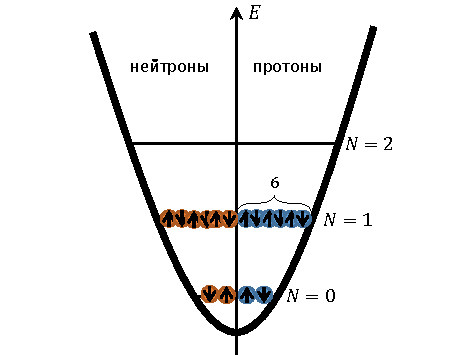
\includegraphics[width=0.7\textwidth,height=\textheight,keepaspectratio]{Seminar_09/pics/pic_parabol_pot.pdf}
    \caption{Структура уровней энергии и их заполнения нуклонами в параболической модели}
    \label{fig:sem_09_parabol_pot}
\end{figure}
Осталось только записать таблички с максимальным количеством заполнения уровней для разных $N$. Вот она:
\begin{table}[H]
\centering
\begin{tabular}{|l|l|l|l|l|}
\hline
\multicolumn{1}{|c|}{$N$} & \multicolumn{1}{c|}{$n_x$, $n_y$, $n_z$}                                                      & \multicolumn{1}{c|}{Всего $p$/$n$} & \multicolumn{1}{c|}{Всего $p+n$} & Элемент    \\ \hline
0                         & (0,0,0)                                                                                       & 2                              & 4                              & $^4_2He$   \\ \hline
1                         & (0,0,1); (0,1,0); (1,0,0)                                                                     & 6                              & 12                             & $^{16}_8O$   \\ \hline
2                         & \begin{tabular}[c]{@{}l@{}}(0,0,2); (0,2,0); (2,0,0)\\ (1,1,0); (1,0,1); (0,1,1)\end{tabular} & 12                             & 24                             & $^{40}_{20}Ca$ \\ \hline
\end{tabular}
\end{table}

Вот таким нехитрым образом в рамках очень простой модели мы получаем те самые <<магические>> стабильные ядра? которые и выбивались на нашем графике удельной энергии связи. Тогда любое излучение или поглощение электромагнитного кванта ядром в рамках данной модели можно рассматривать как переход нуклона в возбужденное состояние на более высокий уровень энергии или релаксацию с него.

Еще один небольшой комментарий про терминологию с которой мы встретимся в задании. Сейчас я написал решение для уровней энергии в таком потенциале для обычных декартовых координат, но эту же задаче можно решить и в сферических координатах. Тогда урони энергии будут называться по другому и совпадать по нотации с уровнями энергии водородоподобного атома, а именно: $N=0 \rightarrow (1S)$, $N=1 \rightarrow (1P)$, $N=2 \rightarrow (1D, 2S)$, $N=3 \rightarrow (1F, 2P)$ и так далее. То есть это просто другое обозначение того же самого и пугаться этого не надо.

\subsection{Радиоактивность. Распады.}
В целом, из школы мы помним, что исторически радиоактивность веществ была открыта супругами Кюри еще в конце 19 века и там получалось 3 разных типа <<излучения>>: $\alpha$ -- вылет ядер гелия, $\beta$ -- вылет электронов,  $\gamma$ обычные фотоны, но с достаточно большой энергией. Естественно есть и более экзотические распады, но их мы рассматривать не будем. Каждые из базовых типов распадов мы рассмотрим более подробно, но предварительно надо написать некоторый общий закон, которой характеризует любые распады с изменением структуры ядра. Тут нам будет достаточно просто базовой логики. Процесс распада квантовый, поэтому там все завязано на вероятности и нам надо написать закон для большого числа части. Процесс распада завязан исключительно на само ядро без его взаимодействия с чем-то еще, то есть это одночастичный процесс. Пользуясь этими 2 фактами мы можем сказать скорость распада будет тем больше, чем больше исходных ядер у нас есть:
\begin{gather*}
\dfrac{dN}{dt} = -\lambda N\\
N(t) = N_0 \exp{(-\lambda t)} = N_0\cdot 2^{-t/T_{1/2}}\\
T_{1/2} = \ln{2} / \lambda
\end{gather*}
$\lambda$ здесь это активность распада или просто число распадов за единицу времени, а $T_{1/2}$ -- это традиционный, известный нам со школы период полураспада. А полную карту характерных распадов можно посмотреть на рисунке \ref{fig:sem_09_isotopes}.

\paragraph{$\alpha$ распад}
Тут из яда вылетает ядро гелия и общая формула для записи распада с количеством нуклонов $A$ и зарядом $Z$: 
\begin{equation*}
    (A,Z) \rightarrow (A-4, Z-2) + He(4,2)
\end{equation*}
Давайте для начала обсудим энергетическую выгодность такого распада. Из рисунка \ref{fig:sem_09_link_energy} видно, что для тяжелых ядер энергия связи на нуклон падает с коэффициентом примерно 1 МэВ на 150 нуклонов, а ядро гели обладает энергией 28 МэВ. Тогда мы можем провести оценку для каких ядер распад возможен:
\begin{gather*}
    E_{\text{св}}(A, Z) < E_{\text{св}}(A-4, Z-2) +28\\
    8A < \left (8 + \dfrac{4}{150} \right) (A-4) + 28\\
    A > 150
\end{gather*}
И это магическим образом совпадает с тем, что мы видим на опыте в рисунке \ref{fig:sem_09_isotopes}. 

Теперь обсудим период полураспада. Для этого достаточно рассмотреть модель туннелирования $\alpha$-частицы из зоны ядра через его кулоновский барьер на свободу. Тут нам поможет формула из 4 семинара и окажется, что если у частицы есть энергия $E_{\alpha}$ то:
\begin{equation}
    \ln{T_{1/2}} \sim -\ln{D} \sim a \dfrac{Z}{\sqrt{E_{\alpha}}} + b
\end{equation}
Это называется законом Гейгера-Неттола. 

Осталось обсудить характерные энергии и спектр $\alpha$-частиц. Диапазон энергий составляет примерно от 4 до 10 МэВ, а спектр альфа частиц всегда линейчатый, что подтверждает, что это внутриядерный процесс без всяких дополнительных извращений.

\paragraph{$\beta$ распад}
На самом деле $\beta$ распад это не обязательно вылет электрона, еще может вылетать позитрон или ядро может захватывать электрон с нижних орбит атома (К-захват). Вот эти три основные формулы:
\begin{gather*}
    (A,Z) \rightarrow (A, Z+1) + e^- + \widetilde{\nu_e}\\
    (A,Z) \rightarrow (A, Z-1) + e^+ + \nu_e\\
    (A,Z) +e^- \rightarrow (A, Z-1) + \nu_e
\end{gather*}

Спектр электронов в отличие от $\alpha$-частиц непрерывный и по энергиям электроны могут достигать 1 МэВ, что делает их релятивистскими. Непрерывность связана с наличие этих самых дополнительных $\nu_e$ или $\widetilde{\nu_e}$ нейтрино или антинейтрино, которые и уносят часть импульса и как раз показывают большую сложность процесса, нежели в случае $\alpha$ распада

\paragraph{$\gamma$ излучение}
Тут нужно понимать, что формально состав ядра при излучении $\gamma$ кванта не меняется, поэтому мы не можем говорить об этом как о распаде, а просто о переходе для ядра из более возбужденного состояния в менее возбужденное или основное. Теперь механизмы возбуждения этого ядра. Бывают однонуклонные, о них мы говорили в рамках оболочечной модели, а бывают коллективные. Представить их себе достаточно просто. Одно из таких возбуждений представлено на рисунке \ref{fig:sem_09_dipole_res}

\begin{figure}[H]
    \centering
    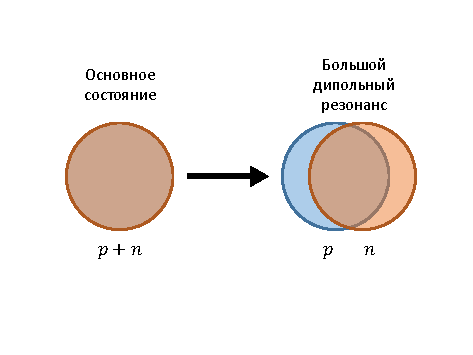
\includegraphics[width=0.6\textwidth,keepaspectratio]{Seminar_09/pics/pic_dipole_resonance.pdf}
    \caption{Пример коллективного возбуждения ядра}
    \label{fig:sem_09_dipole_res}
\end{figure}
Собственно именно такого рода возбуждения и дают нам возможность говорить о E и M фотонах, излучаемых  возбужденным ядром и делают наши оценки вероятности из излучения для атома из прошлого семинара неактуальными.

\section{Практическая часть}
\subsection{Задача 7.5}
\label{task_}
\paragraph{Условие}
С помощью формулы Вайцзеккера найти заряд $Z_0$ наиболее устойчивого ядра-изобары при заданном нечетном значении $A$. Выяснить, каков характер активности у ядер $^{27}Mg$, $^{29}P$, $^{37}K$, $^{67}Cu$.
\paragraph{Решение}
Начнем стандартно с пояснения условия. Что такое ядра-изобары? Это ядра, имеющие одинаковые $A$, но разные символы (разные $Z$), например, $^{14}_6C$ и $ ^{14}_7N$. Теперь что за характер активности? Здесь просто спрашивают а какой распад будет характерен для данных нам ядер. Естественно мы можем посмотреть для каждого из ядер на рисунок \ref{fig:sem_09_isotopes} и по табличке все определить, но давайте разберемся с этим так как и предполагали авторы. У нас есть $\alpha$ и $\beta$ распады (всякую экзотику исключаем). Но массовые числа ядер меньше 150, значит остаются только $\beta$ с вылетом электрона или позитрона. Как определить кто именно вылетит? Просто смотрим какие ядра стабильнее с уменьшением или увеличением заряда. 

Теперь про Вайцзеккера и использование его формулы. Очевидно, что бы найти стабильное ядро нам надо найти локальный максимум энергии связи при данном $A$ и вариации $Z$. Для этого можно просто продифференцировать формулу энергии связи по заряду и приравнять производную к нулю. Я упрощу себе жизнь и возьму $^{27}Mg$. Это четно-нечетное ядро и поэтому последнего члена в формуле Вайцзеккера не будет. Тогда производная:
\begin{gather*}
    \dfrac{dE}{dZ} = -\gamma \dfrac{2Z}{A^{1/3}} + \epsilon \dfrac{(A/2-Z)}{2A} = 0\\
    Z_0 = \dfrac{A/2}{1 + 0.0075 A^{2/3}}
\end{gather*}
 Тогда для магния $^{27}_{12}Mg$ стабильным будет $Z_0=13$ то есть $\beta$ распад должен увеличить заряд на 1, то есть такой магний должен испытать вылет обычного электрона:
 \begin{gather*}
     ^{27}_{12}Mg \rightarrow ^{27}_{13}Al + e^- + \widetilde{\nu_e}
\end{gather*}

\subsection{Задача 7.57}
\label{task_}
\paragraph{Условие}
Нуклон из перезаполненной оболочки ядра углерода $^{13}_6C$, поглощает $E1$-фотон и переходит в возбужденное состояние с наименьшей энергией. Найти спин ядра в конечном состоянии и указать его спектроскопическое обозначение.

\textit{Указание:} Последовательность расположение однонуклонных ядерных уровней $N=0;(1S_{1/2})$, $N=1;(1P_{3/2}, 1P_{1/2})$, $N=2;(2S_{1/2}, 1D_{3/2})$
\paragraph{Решение}
Тут все конечно очень сложно звучит, но на деле это задача на все те же правила отбора, которые у нас были на прошлой неделе, но уже в привязке к ядру, а не к атому. Во-первых, попробуем разобраться с фотоном. Это обычный E1-фотон, значит момент который он уносит это 1 (напомню за момент отвечает чиселко), а то что он электрический означает, что четность этого фотона $(-1)^1 = -1$, значит из закона сохранения четности четность состояний в этом однонуклонном возбуждении должна быть разной (напомню, за четность отвечает механический момент l).

Теперь смотрим на заполнение уровней в оболочечной модели для обычного ${^{12}_6}C$. Уровень $N=0$ или 1S заполнен полностью, а уровень $N=1$ или 1P (здесь $l=1$) заполнен так, чтобы там есть еще 2 места. Значит на него и должен упасть возбужденный нейтрон. А что у нас есть выше? Выше уровень N=2 который неожиданно может быть и 2S (здесь $l=0$) и 1D ($l=2$) Кажется, что нам подходит и то другое, но поскольку от нас спрашивают именно состояние с миимальной энергией, то смотрим на указание и говорим, что нас интересует состояние 2S, а спин тогда будет равен $1/2$, так как один нейтрон у нас нескомпенсированный


\subsection{Комментарии к задачам из задания}
\paragraph{Нулевки} В первой задаче стандартный эффект Доплера, во второй просто баланс энергии и все. Ничего интересного
\paragraph{Задача 7.5} Частично решили, подставьте остальные элементы
\paragraph{Задача 7.16} Как устроены уровни энергии в оболочечной модели  и что такое однонуклонное возбуждение я уже писал, осталось лиши найти характерную частоту осциллятора через глубину ямы
\paragraph{Задача 7.20} Периоды полураспада обратно пропорциональны активностям, а чтобы связь активностей найти нужно записать что происходит с 234 ураном с кинетической точки зрения (за счет чего он появляется и за счет чего уменьшается) и сказать про что-то про стационарность
\paragraph{Задача 7.51} Кажется, что ширина линии однозначно дает время жизни через соотношение неопределнностей, но вот незадача -- ядро после первого излучения гамма кванта движется и работает эффект Доплера
\paragraph{Задача 7.58} Попробуйте использовать рассуждения, аналогичные 7.57
\paragraph{Задача 7.64} Спины протона и нейтрона по $1/2$, но протонов 2 и они спарены, а нейтрон нет. Поэтому надо взять теоретический g-фактор для нейтрона, который равен -3.92

\begin{figure}[h]
    \centering
    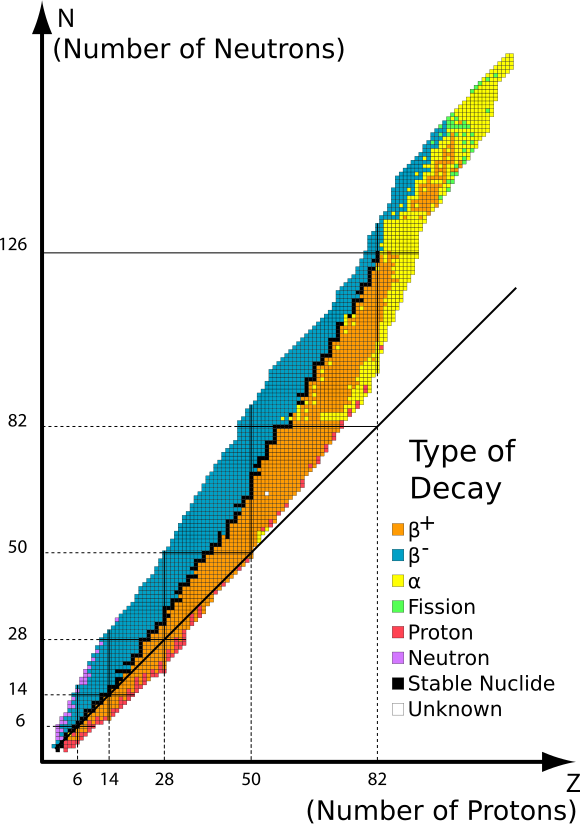
\includegraphics[width=0.8\textwidth,height=\textheight,keepaspectratio]{Seminar_09/pics/pic_table_isotopes.png}
    \caption{Карта характерных распадов для различных ядер}
    \label{fig:sem_09_isotopes}
\end{figure}

\end{document}
